\begin{frame}{Text Classification}
  \centering
  % Title (handled by frame title)

  % TikZ picture for diagram
  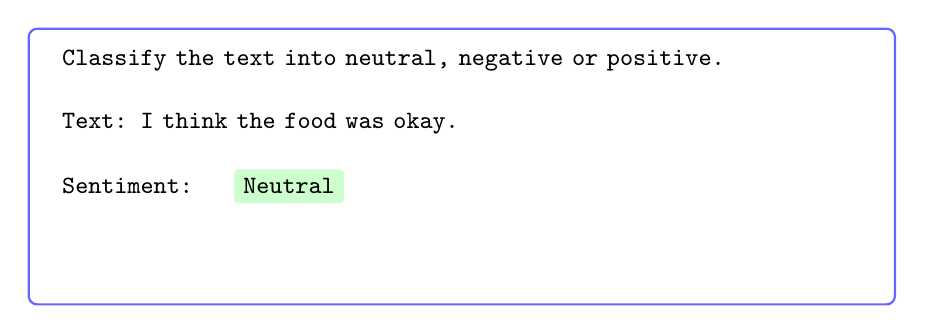
\begin{tikzpicture}
    % Outer blue rounded rectangle
    \draw[thick, rounded corners=3pt, color=blue!60] (0,0) rectangle (11, 3.5);

    % Task instruction (monospaced)
    \node[anchor=west, font=\ttfamily\small, text width=10.5cm] at (0.3, 3.1) {%
      Classify the text into neutral, negative or positive.
    };

    % Text line (monospaced)
    \node[anchor=west, font=\ttfamily\small, text width=10.5cm] at (0.3, 2.3) {%
      Text: I think the food was okay.
    };

    % Sentiment label (highlighted in green)
    \node[anchor=west, font=\ttfamily\small, text width=2.8cm] at (0.3, 1.5) {%
      Sentiment:
    };
    \node[draw=none, fill=green!20, rounded corners=1.5pt, anchor=west, font=\ttfamily\small] at (2.6, 1.5) {Neutral};

  \end{tikzpicture}
\end{frame}
